% Introduction

\chapter{Conformal prediction}

\label{chap:conformal-prediction}

%---------------------------------------
%	SECTION 1: Conformal Prediction (CP)
%---------------------------------------

% \section{Conformal Prediction}\label{sec:cp}

Leveraging same notation as in chapter \ref{chap:intro}, and given $(X, Y)\in \R^d\times\R$ random variables with unknown marginal and joint probability distributions, we want to obtain a $\Ca$ predictive interval. Let us address the case in which $Y=\mu(X) + \epsilon$, where $\mu$ is the model function to be determined and $\epsilon_i\sim P_{Y|X}$ the noise. From now on, we will only assume the data to be \textbf{exchangeable}. 

% For this regression problem we will use the formerly mentioned $n$ samples $(X_i, Y_i)_{i=1}^{n}$, and from now on we will only assume the data to be \textbf{exchangeable}. 

\begin{definition}[Exchangeability]
$\left(X_i, Y_i\right)_{i=1}^n$ are exchangeable if, for any permutation $\sigma$ of $\left[ 1, n \right]$ :
$$
\mathcal{L}\left(\left(X_1, Y_1\right), \ldots,\left(X_n, Y_n\right)\right)=\mathcal{L}\left(\left(X_{\sigma(1)}, Y_{\sigma(1)}\right), \ldots,\left(X_{\sigma(n)}, Y_{\sigma(n)}\right)\right),
$$
where $\mathcal{L}$ designates the joint distribution.
\end{definition}

\begin{example}
    Independent identically distributed (\textit{i.i.d}) samples, or the components of a multidimensional normal distribution, are exchangeable data.
\end{example}
\begin{example}
    Time series data, as well as data obtained from a random variable under any kind of distribution shift, are examples of non-exchangeable data.
\end{example}

Furthermore, as mentioned in section \ref{sec:intro-conformal}, conformal prediction is ultimately based in using the so-called \textit{conformality scores} to construct the predictive interval. These scores, $s_{\Hat{\mu}}$ or directly $s$, allow to transform a heuristic notion of uncertainty from a model $\Hat{\mu}$ into a rigorous measure of it.

Formally, any function $s(X, Y)\in\R$ can be chosen as score if it returns larger values the worse the agreement between $X$ and $Y$ is. Note the choice of conformity score will determine the way confidence intervals are built. 
In particular, the simplest choice is the absolute residual score (namely, the residual) as score for the regression problems: $s_i := s_{\Hat{\mu}}(X_i,Y_i) = \left| Y_i - \Hat{\mu}(X_i) \right|$. 

In this case, then, the predictive intervals is built as 
\begin{equation*}
    \Hat{\Ca} = \left[ 
\Hat{\mu}(X) - q(\mathcal{S}),\ \Hat{\mu}(X) + q(\mathcal{S}) \right],
\end{equation*} where $q(\mathcal{S})$ is the $1-\a$ empirical quantile of the conformity scores $\mathcal{S}=\{s_i\}_{i}$.

\begin{note}
    The \textit{conformity score} election can play a pivotal role in the uncertainty quantification process. In particular, useless or no informative intervals can be obtained in function of the chosen score, as explained in \cite{gentleintro}.
\end{note}

\begin{example}
    There are other well-known scores, for instance those implemented by \cite{mapie:scores}:
    \begin{itemize}
        \item Gamma score $s_{\Hat{\mu}}(X,Y) := \frac{\left| Y - \Hat{\mu}(X) \right|}{\Hat{\mu}(X)}$, such that: \begin{equation*}
            \Hat{\Ca} = \left[ 
\Hat{\mu}(X)\left(1 - q(s)\right),\ \Hat{\mu}(X)\left(1 + q(s)\right) \right]
        \end{equation*}
        \item Residual normalized score $s_{\Hat{\mu}}(X,Y) := \frac{\left| Y - \Hat{\mu}(X) \right|}{\Hat{\sigma}(X)}$, where $\Hat{\sigma}(X)$ is another model which predicts residuals from $X$ (trained on $(X, \left|Y-\Hat{\mu}(X)\right|)$), and it is such that: \begin{equation*}
            \Hat{\Ca} = \left[ 
\Hat{\mu}(X) - q(s)\Hat{\sigma}(X),\ \Hat{\mu}(X) + q(s)\Hat{\sigma}(X)\right]
        \end{equation*}
    \end{itemize}
\end{example}

Within the same conformity score setup, however, several approaches for CP can be applied in function of the user needs regarding computational and statistical efficiency. In this sense, from sections \ref{sec:scp} to \ref{sec:other-flavours}, different CP flavours will be presented; while, in section \ref{sec:cqr}, a way of "\textit{conformalizing}" the quantile regression method is reviewed. Finally, section \ref{sec:guarantees-limits} is devoted the theoretical guarantees and limits of CP and its flavours.

% \subsection{Naive method}

% This approach computes the residuals of the training data to estimate the typical error obtained on a new test data point. Thus, the interval is given by the prediction $\Hat{\mu}(X)$ and adding/subtracting the quantiles of the conformity scores $q(s)$ of the \textbf{same training set}:

% \begin{equation*}
%     \Hat{\Ca}^{\mathrm{naive}}_{n, \a}(X_{n+1}) = \Hat{\mu}(X_{n+1}) \pm \Hat{q}^{+}_{n,\a}(\left|Y_i - \Hat{\mu}(X_i)\right|) =: \Hat{\mu}(X_{n+1}) \pm \Hat{q}^{+}_{n,\a}(s_i), 
% \end{equation*} if we set $s_i:=\left|Y_i - \Hat{\mu}(X_i)\right|$ from now on.

% Of course, however, this method does not attain valid statistical coverage and underestimates the width of prediction intervals because of a potential overfit (the conformity scores are estimate only on the training set).

\section{Split Conformal Prediction}\label{sec:scp}

Split Conformal Prediction (SCP) is the most widely-used flavour of conformal prediction and it is based in splitting the data in a training $\mathrm{Tr}$ set and a calibration $\mathrm{Cal}$ set. Thus, if we used the absolute residual as conformity score, SCP would prescribe as it follows:

\begin{enumerate}
    \item Split the data set into a \textbf{training set} of size $\#\mathrm{Tr}$ and a \textbf{calibration set} of size $\#\mathrm{Cal}$
    \item Obtain $\Hat{\mu}$ by training the algorithm in the $\mathrm{Tr}$ set
    \item Obtain a set $\S$ of conformity scores by using the $\mathrm{Cal}$ set: $\S_{\mathrm{Cal}}:=\{ s_i \}_{i\in \mathrm{Cal}}=\{ \left|Y_i - \Hat{\mu}(X_i)\right|, i\in \mathrm{Cal}\}$
    \item Compute $q_{1-\a^{\mathrm{SCP}}}(\S_{\mathrm{Cal}})$, namely the $(1-\a)\left(\frac{1}{\#\mathrm{Cal}}+1\right)$ quantile of $\S_{\mathrm{Cal}}$. From now on, we will indistinctly write $q_{1-\a^{\mathrm{SCP}}}(\S_{\mathrm{Cal}})\equiv q_{1-\a}(\S_{\mathrm{Cal}})$
    \item For a new sample $X_{n+1}$, return the predictive interval
    \begin{equation}
        \label{eq:scp}
        \Hat{\Ca} = \left[\Hat{\mu}(X_{n+1}) - q_{1-\a}(\S_{\mathrm{Cal}}),\ \Hat{\mu}(X_{n+1}) + q_{1-\a}(\S_{\mathrm{Cal}})\right]
    \end{equation}
\end{enumerate}

\begin{note}
    To attain at least $1 - \a$ coverage taking into account the finite number of samples in the $\mathrm{Cal}$ set, in step 4 the quantile of conformity scores $q_{1-\a^{\mathrm{SCP}}}(\S)\equiv q_{1-\a}(\S)$ must be computed as a $(1-\a)\left(\frac{1}{\#\mathrm{Cal}}+1\right)$-quantile (instead of a $(1-\a)$-quantile), the so-called \textbf{$1-\a$ empirical quantile}.
\end{note}

Let us, in Algorithm \ref{alg:SCP}, state the algorithm independently of the conformity score $s$ choice.

\begin{algorithm}
\caption{SCP algorithm}\label{alg:SCP}
\begin{algorithmic}[1] 
\REQUIRE Regression algorithm $\A$, miscoverage level $\a$, data samples $\{\left(X_t,Y_t\right)\}^T_{t=1}$. 
\ENSURE Prediction interval $\Ca(X) \text { for any } X \in \R^d$. 
\STATE Randomly split $\{1, \ldots, T\}$ into two disjoint sets $\mathrm{Tr}$ and $\mathrm{Cal}$. 
\STATE Fit a mean regression function: $\hat{\mu}(\cdot) \leftarrow \mathcal{A}\left(\left\{\left(X_t,Y_t\right), t \in \mathrm{Tr}\right\}\right)$. 
\FOR {$j \in \mathrm{Cal} $} 
\STATE Set $s_j$ the \textit{conformity scores}. 

\hspace{4mm} Note if we chose \textit{e.g.} the absolute residual as conformity score, then $s_j := s_{\Hat{\mu}}(X_j, Y_j) = |Y_j-\hat{\mu}(X_j)|$.

\ENDFOR
\STATE Set $\S_{\mathrm{Cal}} = \{s_j, j\in \mathrm{Cal}\}$.
\STATE Compute $q_{1-\a}\left(\S_{\mathrm{Cal}}\right)$, the $(1-\a )\left(1+1/\left|\mathrm{Cal}\right|\right)$ quantile of $\S_{\mathrm{Cal}}$ (\textit{i.e.} the $1-\a$ empirical quantile).
\STATE Return $\Ca(X) = \{Y \in \R\ |\ s_{\Hat{\mu}}(X, Y) \leq q_{1-\a}(\S_{\mathrm{Cal}}) \}$, for any $X \in \R^d$. 

\hspace{4mm} Note the explicit form of $\Ca(x)$ depends on the conformality score; \textit{e.g.} if we chose the absolute residual, then $\Ca(X) = \left[\hat{\mu}(X)\pm q_{1-\a}\left(\S_{\mathrm{Cal}}\right)\right]$.

\end{algorithmic}
\end{algorithm}

Notice SCP requires that one must have enough observations to split its original dataset into train and calibration, but at least it attains the expected coverage of $\geq 1 -\a$. This will be theoretically backed later at section \ref{guarantees:scp}, particularly through Theorem \ref{thm:scp}.

\section{Full Conformal Prediction}\label{sec:fcp}

Even though SCP attains expected coverage and just needs to fit a model $\mu$ once (thus, it is not computationally demanding), the dataset needs to be large enough for $\Ca$ to be informative. 

Full Conformal Prediction (FCP) is born as a workaround to this problem. Unlike SCP, FCP leverages the whole dataset as training and its core idea is as stated at \cite{gentleintro}.\\

Let us assume the dataset $\{(X_t, Y_t)\}_{t=1}^{T}$ is available and, for a new sample $X_{T+1}$, the user wants to provide the interval $\Ca(X_{T+1})$. Then, since the true label $Y_{T+1}$ lies somewhere in $\mathcal{Y} := \mathrm{Im}(\mu)\subset\R$, looping over all possible $Y\in\mathcal{Y}$ will eventually hit in the $(X_{T+1}, Y_{T+1})$ data point which is exchangeable with the first $T$ points; specifically, the most probable labels will have a low enough conformity score.\\

FCP, as explained in Algorithm \ref{alg:FCP}, consists in: "\textit{discretizing}" the target space $\mathcal{Y}$ into $N$ candidates $Y_j$, traversing this loop fitting the estimator to the data \& $(X_{T+1},Y_{j})$ as new data point, and finally returning those candidates $Y_{j}$ such that they "conform enough" to the data. The latter condition will be translated to asserting whether the conformity score of $Y_{j}$ candidate is "low enough" (lower than the $1-\alpha$ empirical quantile of all conformity scores $\mathcal{S}$).\\

\begin{algorithm}
\caption{FCP algorithm}\label{alg:FCP}
\begin{algorithmic}[1] 
\REQUIRE Regression algorithm $\A$, miscoverage level $\a$, data samples $\{\left(X_t,Y_t\right)\}^T_{t=1}$ and new $X_{T+1}$ feature sample. 
\ENSURE Prediction interval $\Ca(X_{T+1}) \text { for any given } X_{T+1} \in \R^d$. 
\STATE Discretize the target space $\mathcal{Y}$ reducing into $N$ candidates $Y_j$. 
\STATE Initialize $\Hat{\mathcal{Y}}_{\mathrm{low}} = \{\}$ the array for candidates with "low enough" conformity score
\FOR {$j \in \{1, \ldots, N\},\ Y_j$ candidate} 
\STATE Fit a mean regression function $\mu_j$ using $\mathrm{Tr}_j=\{\left(X_t,Y_t\right)\}^T_{t=1}\cup \{(X_{T+1}, Y_j)\}$ as training data: $$\hat{\mu}_j(\cdot) \leftarrow \mathcal{A}\left(\left\{\left(X_t,Y_t\right), t \in \mathrm{Tr}_j\right\}\right)\ .$$
\STATE Set $\S_j=\{ s_{\Hat{\mu}_j}(X_i, Y_i) \}_{i=1}^T\cup \{s_{\Hat{\mu}_j}(X_{T+1}, Y_j)\}$ the conformity scores obtained in the same $\mathrm{Tr}_j$ training data.
\STATE Set $q^j_{1 - \a}(\S_{j})$ the $(1-\a )\left(1+\frac{1}{T+1}\right)$ quantile of $\S_{j}$ (\textit{i.e.} the $1-\a$ empirical quantile)
\IF {$s_{\Hat{\mu}_j}(X_{T+1}, Y_j) \leq q^j_{1 - \a}(\S_{j})$}
\STATE Add $Y_j$ to $\Hat{\mathcal{Y}}_{\mathrm{low}}$
\ENDIF

\ENDFOR
\STATE Return $\Ca(X_{T+1}) = \Hat{\mathcal{Y}}_{\mathrm{low}}$.

\end{algorithmic}
\end{algorithm}

Note FCP solves the problem of effectively reducing the dataset through a split, at expenses of a huge computational efforts. In particular, FCP requires to re-fit the model $N$ times for every new $X_{T+1}$ feature sample.

Of course, the existence of $N$ is due to the fact we need to discretize $\mathcal{Y}$ to compute $\Ca(X_{T+1})$. In this sense, the larger $N$ the more accurate FCP will be, but then the more time it will take to infer the predictive set. 

Notice that in the non-discrete case (\textit{i.e.} when $N\rightarrow+\infty$) we would be returning the continuous set $$\Ca(X_{T+1}) = \{Y \in\R\ |\ s_{\Hat{\mu}_j}(X_{T+1}, Y) \leq q^j_{1 - \a}(\S_{j}) \}\ .$$

\section{Other flavours}\label{sec:other-flavours}

On the one hand, in \ref{sec:scp} it is shown split conformal prediction requires only one model fitting step, but sacrifices statistical efficiency. On the other hand, in \ref{sec:fcp} is reviewed how full conformal prediction requires a very large number of model fitting steps, but has high statistical efficiency. These are not the only two achievable points on the spectrum: but there are techniques that precisely fall in between, trading off statistical efficiency and computational efficiency differently.

As represented in Figure \ref{fig:trade-off}, this is the case of cross-conformal prediction CV+ (\cite{vovk2015}) and Jackknife+ (\cite{barber2021b}), methods which both use a small number of model fits, but still leveraging all data for both model fitting and calibration.\\

\begin{figure}%[h]
    \centering
    % \includegraphics{}
    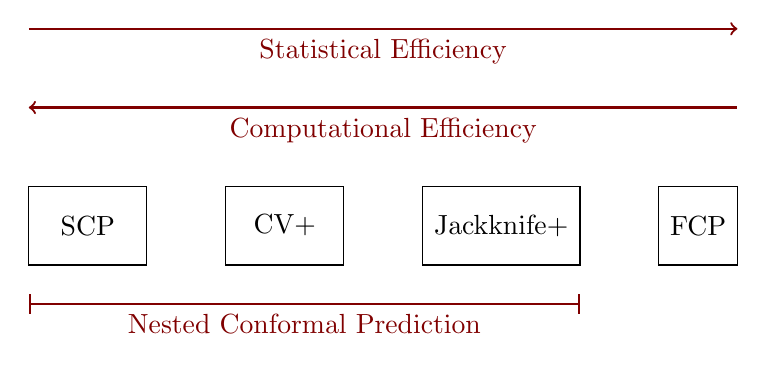
\begin{tikzpicture}
        \definecolor{tred}{HTML}{800000}
        % Draw the horizontal arrows
        \draw[thick, ->, tred] (1, 0) -- (10, 0) node[anchor=north, pos=0.5] {Statistical Efficiency};
        \draw[thick, <-, tred] (1, -1) -- (10, -1) node[anchor=north, pos=0.5] {Computational Efficiency};
        % Draw the boxes
        \draw (1, -3) rectangle (2.5, -2) node[pos=0.5] {SCP};
        \draw (3.5, -3) rectangle (5, -2) node[pos=0.5] {CV+};
        \draw (6, -3) rectangle (8, -2) node[pos=0.5] {Jackknife+};
        \draw (9, -3) rectangle (10, -2) node[pos=0.5] {FCP};
        % Draw the nested conformal prediction arrow
        \draw[thick, |-|, tred] (1, -3.5) -- (8, -3.5) node[anchor=north, pos=0.5] {Nested Conformal Prediction};
    \end{tikzpicture}

    \caption{Representation of the trade-off between statistical and computational efficiencies for the different approaches. Based on \cite{cptuto}.}
    \label{fig:trade-off}
\end{figure}

On the one hand, the so-called Jackknife+ method is based on leave-one-out (LOO) and, for a new $X_{n+1}$, it heuristically prescribes:
\begin{enumerate}
    \item For each $i\in\mathcal{D}:=\{1,\ldots, T\}$ sample of the training data:
    \begin{itemize}
        \item Fit a mean regression function $\mu_{-i}$ training $\mathcal{A}$ in $\mathcal{D}\setminus (X_i, Y_i)$: $$\hat{\mu}_{-i}(\cdot) \leftarrow \mathcal{A}\left(\left\{\left(X_t,Y_t\right), t \in \mathcal{D}\setminus (X_i, Y_i)\right\}\right)\ .$$
        \item Get the conformity scores $$\S^i_{\mathrm{up/down}} = \hat{\mu}_{-i}(X_{n+1}) \pm s_{\hat{\mu}_{-i}}(X_i, Y_i) $$
    \end{itemize}
    \item Set the conformity scores' sets: $\S_{\mathrm{up}} = \{\S^i_{\mathrm{up}}\}_{i\in\mathcal{D}}$ and $\S_{\mathrm{down}} = \{\S^i_{\mathrm{down}}\}_{i\in\mathcal{D}}$
    \item Defining $q_{\beta,\mathrm{inf}}(Z_1, \ldots,Z_n)$ as the $\lfloor\beta\times n\rfloor$ smallest value of $(Z_1, \ldots,Z_n)$, and $q_{1-\a}$ the $1-\a$ empirical quantile; the following predictive interval is returned: $$ \Hat{\Ca}(X_{n+1}) = \left[q_{\a,\mathrm{inf}}(\S_{\mathrm{down}}),\ q_{1-\a}(\S_{\mathrm{up}})\right] $$
\end{enumerate}

Note, however, J$+$aB may be more computationally demanding even than FCP if the dataset is large such $T>N$ (more samples $T$ than $N$ points needed to \textit{discretize} the $\mathcal{Y}$ space in FCP). 

On the other hand, the CV+ method is based on cross-validation residuals and precisely extends the previous idea into a "batch" of samples. Thence, the following differences must be taken into account:
\begin{itemize}
    \item Instead of leaving one out of $\mathcal{D}$,  CV+ splits the data into $K$ folds $F_1,\ldots, F_K$.
    \item Then, for each $k\in\{1,\ldots, K\}$ fold:
    \begin{itemize}
        \item A mean regression function $\mu_{-{F_K}}$ is fit training $\mathcal{A}$ in $\mathcal{D}\setminus F_k$, instead of $\mathcal{D}\setminus (X_i, Y_i)$.
        \item The conformity scores are no longer a value (for each $i\in\{1,\ldots,N\}$) but a subset (obtained with samples within each fold $k$): $$\S^k_{\mathrm{up/down}} = \{\hat{\mu}_{-k}(X_{n+1}) \pm s_{\hat{\mu}_{-k}}(X_i, Y_i)\}_{i\in F_k} $$
    \end{itemize}
\end{itemize}

Notice this method enhances the computational efficiency at expenses of the statistical's, by training $\A$ less times (and with less data). For a precise and complete description of the algorithms, we refer the reader to the former works (\cite{vovk2015} and \cite{barber2021b}).

%---------------------------------------
%	SECTION 1: Conformalized QR (CQR)
%---------------------------------------

\section{Conformalized Quantile Regression}\label{sec:cqr}

While the former flavours of conformal prediction have theoretical guarantees for its statistical coverage, just marginal coverage is sought thus providing non-adaptive predictive intervals: $$ \mathbb{P}\left\{Y_{n+1} \in \Hat{\Ca}\left(X_{n+1}\right) \cancel{ \mid X_{n+1}=x }\right\} \geq 1-\a $$

In this section, thence, we present the Conformalized Quantile Regression (CQR) as means of obtaining more adaptive intervals $\Ca$. As discussed in \ref{guarantees:limits}, notice that while approximate and asymptotic conditional coverage can be sought, conformal prediction (even within CQR) does not guarantee it without further assumptions than data exchangeability. Nevertheless, at practice, CQR will allow us to obtain more informative intervals.\\

CQR proposes to fit not one $\mu$ but two models $\mu_{\mathrm{down}}$ and $\mu_{\mathrm{up}}$ and adjusting the conformality score $s_{\mu}$ to: \begin{equation}\label{eq:cqr-score}
    s_{\A}(X_i,Y_i):=\mathrm{max}\left( {\hat{\mu}}_{\mathrm{down}}(X_i) - Y_i,\ Y_i - {\hat{\mu}}_{\mathrm{up}}(X_i)\right)
\end{equation}

The model $\mu_{\mathrm{down}}$ and $\mu_{\mathrm{up}}$ are no longer trying to capture the mean value of $(X,Y)$, but rather the low and high quantiles of their distribution (\textit{e.g.} $\mu_{\mathrm{down}}$ \& $\mu_{\mathrm{up}}$ could be estimators of the $\a/2$ and $1-\a/2$ quantiles). In this sense, CQR achieve adaptive predictive intervals by adding/subtracting the conformity score to the inferred values of 2 different estimators.

Thus, CQR is not a different methodology but another "choice" of conformity score definition and it is compatible with the SCP or FCP approaches (or others such as Jackknife+, CV+...). 

Let us see, as an example in Algorithm \ref{alg:CQR}, what CQR prescribes if we use the SCP approach:

\begin{algorithm}
\caption{CQR algorithm (using split prediction)}\label{alg:CQR}
\begin{algorithmic}[1] 
\REQUIRE Regression algorithm $\A$, miscoverage level $\a$, data samples $\{\left(X_t,Y_t\right)\}^T_{t=1}$. 
\ENSURE Prediction interval $\Ca(X) \text { for any } X \in \R^d$. 
\STATE Randomly split $\{1, \ldots, T\}$ into two disjoint sets $\mathrm{Tr}$ and $\mathrm{Cal}$. 
\STATE Fit 2 regression functions, one for the lower quantile $\hat{\mu}_{\mathrm{down}}$ and one for the upper $\hat{\mu}_{\mathrm{up}}$: $$\hat{\mu}_{\mathrm{down}}(\cdot), \hat{\mu}_{\mathrm{up}}(\cdot) \leftarrow \mathcal{A}\left(\left\{\left(X_t,Y_t\right), t \in \mathrm{Tr}\right\}\right)\ .$$ 
\vspace{-4mm}

\FOR {$j \in \mathrm{Cal} $} 
\STATE Set $s_j$ the \textit{conformity score} using \ref{eq:cqr-score}: $$s_j := s_{\A}(X_j, Y_j)=\mathrm{max}\left(\hat{\mu}_{\mathrm{down}}(X_i) - Y_i,\ Y_i - \hat{\mu}_{\mathrm{up}}(X_i)\right)$$ 
\vspace{-5mm}
\ENDFOR
\STATE Set $\S_{\mathrm{Cal}} = \{s_j, j\in \mathrm{Cal}\}$.
\STATE Compute $q_{1-\a}\left(\S_{\mathrm{Cal}}\right)$, the $(1-\a )\left(1+1/\left|\mathrm{Cal}\right|\right)$ quantile of $\S_{\mathrm{Cal}}$ (\textit{i.e.} the $1-\a$ empirical quantile).
\STATE Return $\Ca(X_{n+1}) = \left[\hat{\mu}_{\mathrm{down}}(X_{n+1}) - q_{1-\a}\left(\S_{\mathrm{Cal}}\right),\ \hat{\mu}_{\mathrm{up}}(X_{n+1}) + q_{1-\a}\left(\S_{\mathrm{Cal}}\right)\right]$ for any new $X_{n+1} \in \R^d$. 
\end{algorithmic}
\end{algorithm}

%%%%%%%%%%%%%%%%%%%%%%%%%%%%%%%%%%%%%%%%%%%%%%%%%%%%%%%%%%%%%%%

\section{Theoretical guarantees and limits}\label{sec:guarantees-limits}

Even though the heuristic notion justifying the validity of the different paradigms of conformal prediction may be clear, we have not discussed its theoretical guarantees and limits yet. Yet, this is precisely the objective in this section: while in \ref{guarantees:scp} and \ref{guarantees:fcp} we will proof $1-\a$ coverage can be sought in SCP and FCP respectively, in \ref{guarantees:others} we will discuss which are the guarantees for Jackknife+ and CV+, and we will conclude by reviewing the known limits of conformal prediction in \ref{guarantees:limits}.

\subsection{Split Conformal Prediction}\label{guarantees:scp}

Henceforth, in Theorem \ref{thm:scp} and through Lemma \ref{lemma:quantile}, the theoretical guarantee of SCP (algorithm \ref{alg:SCP}) is proven. We reproduce the proof found at \cite{cptuto}, which is general for any conformity score $s$ choice; however, note that:
\begin{itemize}
    \item The proof for the lower bound initially appeared at \cite{papadopoulos} for \textit{i.i.d.} data. Then, \cite{vovk2005} proved that the theorem also holds if the observations satisfy the weaker condition of exchangeability.
    \item The upper bound case was initially proved with Theorem 2.2 of \cite{lei2018} (along the lower bound case, see A.1) but specifically for the absolute residual score case. The proof required the residuals to have a continuous joint distribution, but as mentioned in \cite{gentleintro} this condition is not important because the user can always add a vanishing amount of random noise to the score. 
    \item Both lower and upper bound cases were later stated for the CQR case in Theorem 1 of \cite{romano2019} (and proved in its supplementary material).
\end{itemize}

\begin{lemma}[Quantile lemma]\label{lemma:quantile}
    If $\left(U_1, \ldots, U_n, U_{n+1}\right)$ are exchangeable, then for any $\left.\beta \in\right] 0,1[$: $$ \mathbb{P}\left(U_{n+1} \leq q_\beta\left(U_1, \ldots, U_n,+\infty\right)\right) \geq \beta . $$
    Additionally, if $U_1, \ldots, U_n, U_{n+1}$ are almost surely distinct, then:
$$ \mathbb{P}\left(U_{n+1} \leq q_\beta\left(U_1, \ldots, U_n,+\infty\right)\right) \leq \beta+\frac{1}{n+1} $$
\end{lemma}
\begin{proof}
    First note that $U_{n+1} \leq q_\beta\left(U_1, \ldots, U_n,+\infty\right) \Longleftrightarrow U_{n+1} \leq q_\beta\left(U_1, \ldots, U_n, U_{n+1}\right)$.
Then, by definition of $q_\beta$ :
$$
U_{n+1} \leq q_\beta\left(U_1, \ldots, U_n, U_{n+1}\right) \Longleftrightarrow \operatorname{rank}\left(U_{n+1}\right) \leq\lceil\beta(n+1)\rceil
$$

By exchangeability, $\operatorname{rank}\left(U_{n+1}\right) \sim \mathcal{U}\{1, \ldots, n+1\}$. Thus:
$$
\mathbb{P}\left(\operatorname{rank}\left(U_{n+1}\right) \leq\lceil\beta(n+1)\rceil\right) \geq \frac{\lceil\beta(n+1)\rceil}{n+1} \geq \beta .
$$

If $U_1, \ldots, U_n, U_{n+1}$ are almost surely distinct (without ties):
$$
\begin{aligned}
\mathbb{P}\left(\operatorname{rank}\left(U_{n+1}\right) \leq\lceil\beta(n+1)\rceil\right) & =\frac{\lceil\beta(n+1)\rceil}{n+1} \\
& \leq \frac{1+\beta(n+1)}{n+1}=\beta+\frac{1}{n+1} . \end{aligned}
$$
\end{proof}

% proof for SCP's guarantees
\begin{theorem}[SCP guarantees]\label{thm:scp}
    Suppose $\left(X_i, Y_i\right)_{i=1}^{n+1}$ are exchangeable. SCP applied on $\left(X_i, Y_i\right)_{i=1}^n$ yields $\Hat{\Ca}(\cdot)$ such that:
$$ \mathbb{P}\left\{Y_{n+1} \in \Hat{\Ca}\left(X_{n+1}\right)\right\} \geq 1-\a . $$

Additionally, if the scores $\left\{S_i\right\}_{i \in \mathrm{Cal}} \cup\left\{S_{n+1}\right\}$ are a.s. distinct: $$
\mathbb{P}\left\{Y_{n+1} \in \Hat{\Ca}\left(X_{n+1}\right)\right\} \leq 1-\a+\frac{1}{\# \mathrm{Cal}+1}
$$
\end{theorem}
\begin{proof}
    When $\left(X_i, Y_i\right)^{n+1}_{i=1}$ are exchangeable, the scores $\{S_i\}_{i\in\mathrm{Cal}}\cup \{S_{n+1}\}$ are also exchangeable. Applying Lemma \ref{lemma:quantile} to the scores concludes the proof.
\end{proof}

\subsection{Full Conformal Prediction}\label{guarantees:fcp}

Even though it leverages all data samples, FCP also attains the expected $1-\a$ statistical coverage and the idea in which the proof relies is really similar to the SCP proof (in particular, it strongly relies on the exchangeability of the $s_{n+1}$ conformity score \textit{w.r.t.} $s_{1},\ldots,s_{n}$). 

However, an additional hypothesis is needed and, although related to exchangeability, consists in the algorithm $\A$ being \textit{symmetrical}.  

\begin{definition}[Symmetrical algorithm]
A deterministic algorithm $\A: \left(U_1, \ldots, U_n\right)\rightarrow\hat{A}$ is symmetric if, for any permutation $\sigma$ of $\left[ 1, n \right]$ :
$$ \mathcal{A}\left(U_1, \ldots, U_n\right)\myeq 
 \mathcal{A}\left(U_{\sigma(1)}, \ldots,U_{\sigma(n)}\right)\ .$$
\end{definition}

With this new restraint, the following theorem can now be announced:

% proof for FCP's guarantees
\begin{theorem}[FCP guarantees]\label{thm:fcp}
    Suppose $\left(X_i, Y_i\right)_{i=1}^{n+1}$ are exchangeable and $\A$ is symmetric. FCP applied on $\left(X_i, Y_i\right)_{i=1}^n\cup \{X_{n+1}\}$ yields $\Hat{\Ca}(\cdot)$ such that:
$$ \mathbb{P}\left\{Y_{n+1} \in \Hat{\Ca}\left(X_{n+1}\right)\right\} \geq 1-\a . $$

Additionally, if the scores are a.s. distinct: $$
\mathbb{P}\left\{Y_{n+1} \in \Hat{\Ca}\left(X_{n+1}\right)\right\} \leq 1-\a+\frac{1}{n+1}
$$
\end{theorem}

For sake of length and in view of the similarity of FCP proof \textit{w.r.t.} to SCP's, Theorem \ref{thm:fcp} proof will be skipped. Nevertheless, for a detailed version, the reader can refer to \cite{vovk2005} or \cite{lei2018} (A.1 appendix proof of Theorem 2.1). % see https://arxiv.org/pdf/1604.04173.pdf

% \textcolor{red}{En el teorema de la secció 6.1 de \url{https://arxiv.org/pdf/2107.07511.pdf} citen Vovk 2005.}

\subsection{Other flavours}\label{guarantees:others}

Whereas SCP sacrificed statistical efficiency at expenses of computational efforts by splitting the available dataset in two, FCP proposed the contrary leveraging all the data but at the price of much more model fits; and, so far, we have seen these both two opposite methodologies guarantee $1-\a$ statistical coverage.

In this section, we briefly discuss the state of 2 approaches in-between the spectrum: the Jackknife+ \& the CV+.\\

In this sense, in general, it is seen the Jackknife+ method does not guarantee $1-\a$ statistical coverage. Nevertheless, as proved in \cite{barber2021b}, if $\{(X_i, Y_i)\}_{i=1}^{n+1}$ are exchangeable and $\mathcal{A}$ symmetric, then: $$ \mathbb{P}\left(Y_{n+1}\in \Hat{\Ca}(X_{n+1})\right) \geq 1 - 2\a$$

Yet, \cite{barber2021b} proposes the so-called "\textit{jackknife-minmax}" method to attain $1-\a$ coverage within the jackknife setting; in practice, it is seen the yielded prediction intervals are too conservative.\\

We can refer to the same former reference to find out the CV+ method, proposed in \cite{vovk2015}, is another case in which $1-\a$ coverage is no attained without further assumptions.

Actually, within the same hypothesis of $\{(X_i, Y_i)\}_{i=1}^{n+1}$ being exchangeable and $\mathcal{A}$ symmetric, one can prove that, for CV+:
 $$ \mathbb{P}\left(Y_{n+1}\in \Hat{\Ca}(X_{n+1})\right) \geq 1 - 2\a - \mathrm{min}\left(\frac{2\left(1 - 1/K\right)}{n/K + 1}, \frac{1 - K/n}{K + 1}\right) \geq 1 - 2\alpha - \sqrt{2/n}$$

It is beyond the scope of this work offer complete proof for these results; however, to obtain an exhaustive overview, the user is referred to \cite{barber2021b}.

\subsection{Impossibility results}\label{guarantees:limits}

So far, it has been shown SCP (and FCP) just requires data exchangeability (as well as $\A$ to be symmetrical) in order to achieve guaranteed $1-\a$ statistical coverage. 

Of course, even though useful and informative predictive intervals can be obtained (precisely, this is the purpose of CP), the type of coverage we can expect is marginal rather than conditional.\\

This is precisely the impossibility result \cite{lei2014}; \cite{vovk2012} and \cite{barber2021a} have reached to: without distribution assumption, in finite sample, a perfectly conditionally valid $\Hat{\Ca}$ is such that $\mathbb{P}\left\{\operatorname{mes}\left(\Hat{\Ca}(x)\right)=\infty\right\}=1$ for any non-atomic $x$. Namely, the measure of $\Hat{\Ca}(x)$ will be, with all probability, infinite.\\
    
However, for certain problems and in function of the sample size, approximate or even asymptotic conditional coverage can be reached. Below, several of these results are cited so that the user can refer to them: 
\begin{itemize}
\item \textbf{Approximate conditional coverage}: $\mathbb{P}\left(Y_{n+1} \in \Hat{\Ca} \mid X_{n+1} \in \mathcal{R}(x)\right) \geq 1-\a$ for certain $\mathcal{R}(x)$ clusters or aggregations of the features samples.
\begin{itemize}
    \item \cite{romano2020a}: in classification problems, approximate conditional coverage can be sought for specialized versions of Jackknife+ and CV+ techniques and categorical \& unordered response labels.
    \item \cite{guan2022}: additional local coverage guarantees (under suitable assumptions) by offering a single-test-sample adaptive construction that emphasizes a local region around this test sample.
    \item \cite{jung2022}: CP algorithms are proposed in order to attain multivalid coverage on exchangeable data in the batch setting (a little bit stronger than conditional coverage on group membership).
    \item \cite{gibbs2023}: reformulates conditional coverage as coverage over a class of covariate shifts and, when the target class of shifts is finite dimensional, finite sample coverage over all possible shifts is achieved.
\end{itemize} 
\item \textbf{Asymptotic (with the sample size) conditional coverage}: 
\begin{itemize}
    \item \cite{kivaranovic2020a}: a neural network is proposed so that it outputs three values instead of a single point estimate and optimizes a loss function motivated by the standard quantile regression loss, achieving stronger coverage. 
    \item \cite{izbicki2020a} and \cite{izbicki2022}: both introduce some conformal methods based on conditional density estimators to obtain asymptotic conditional coverage; most based on the idea of creating prediction bands (in a data-driven way) locally on a partition of the features space.
    \item \cite{chernozhukov2021}: a method is proposed to construct conditionally valid prediction intervals based on models for conditional distributions (such as quantile and distribution regression).
    \item \cite{sesia2021}: a conformal method is proposed to compute prediction intervals for non-parametric regression that can automatically adapt to skewed data (with probably marginal coverage in finite samples, while asymptotically achieving conditional coverage if the model is consistent).
\end{itemize}
\end{itemize}
